\documentclass[12pt]{article}
\usepackage{graphicx}
\usepackage{amsmath}
\usepackage{latexsym}
\usepackage{amstext}
\usepackage{array}
\usepackage{multirow}
\usepackage{stackrel}
\usepackage{caption}
\usepackage{subcaption}

%%%%%%%%%%%%%%%%%%%%%%%%%%%%%%%%%%%%%%%%%%%%%%%%%%%%%%%%%%%%%%%%%%%%%%%%%%%=
\newtheorem{proposition}{Proposition}
\newtheorem{lemma}{Lemma}
\newtheorem{theorem}{Theorem}
\newtheorem{corollary}{Corollary}
\newcommand{\Proof}{\underline{\bf Proof:}}
\newcommand{\Endproof}{~$\Box$~}
\newcommand{\mb}[1]{ \mbox{\boldmath$#1$} }
\newcommand{\ds}{\displaystyle}
\newcommand{\beq}{\begin{eqnarray}}
\newcommand{\eeq}{\end{eqnarray}}
\newcommand{\beqq}{\begin{eqnarray*}}
\newcommand{\eeqq}{\end{eqnarray*}}
\newcommand{\p}{\partial}
\newcommand{\g}{\gamma}
\newcommand{\eps}{\varepsilon}
\newcommand{\x}{\mbox{\boldmath$x$}}
\newcommand{\n}{\mbox{\boldmath$n$}}
\newcommand{\J}{\mbox{\boldmath$J$}}
%\newcommand{\v}{\mbox{\boldmath$v$}}
\newcommand{\y}{\mbox{\boldmath$y$}}
\newcommand{\z}{\mbox{\boldmath$z$}}
\font\bb=msbm10 at 12pt
\def\rR{\hbox{\bb R}}
\def\rN{\hbox{\bb N}}
\def\rQ{\hbox{\bb Q}}
\def\rZ{\hbox{\bb Z}}
\pagestyle{plain}
%%%%%%%%%%%%%%%%%%%%%%%%%%%%%%%%%%%%%%%%%%%%%%%%%%%%%%%%%%%%%%%%%%%%%%%%%%%%
\begin{document}

\title{Chromatin reconstruction and dynamics using random Loops accounting for Chromosome Capture data}
\author{O. Shukron,  L. Giogetti, E. Heard and D. Holcman$^{1}$ \footnote{ $^1$Ecole Normale Sup\'erieure, IBENS, 46 rue d'Ulm 75005 Paris, France.}}
\date{\today}
\maketitle
%%%%%%%%%%%%%%%%%%%%%%%%%%%%%%%%%%%%%%%%%%%%%%%%%%%%%%%%%%%%%%%%%%%%%%5
\begin{abstract}\label{abstract}
\end{abstract}
{\bf \noindent Keywords: Modeling, Inverse problem, First passage times,}\\

\section{Introduction}\label{section_introduction}

\section{Experimental data and Methods}\label{section_experimentalDataAndMethods}

\subsection{The experimental data}\label{subsection_theExperimentalData}

\subsection{The polymer model}\label{subsection_thePolymerModel}

\subsection{Simulations}\label{subsection_simulations}

\section{Results}\label{section_results}

\subsection{Analysis of the experimental data}\label{subsection_analysisOfTheExperimentalData}

\subsection{Random fixed loops simulations}\label{subsection_randomFixedLoopsSimulations}

\section{Discussion}\label{section_discussion}

\section{Figure}\label{section_figures}

\begin{figure}[H]
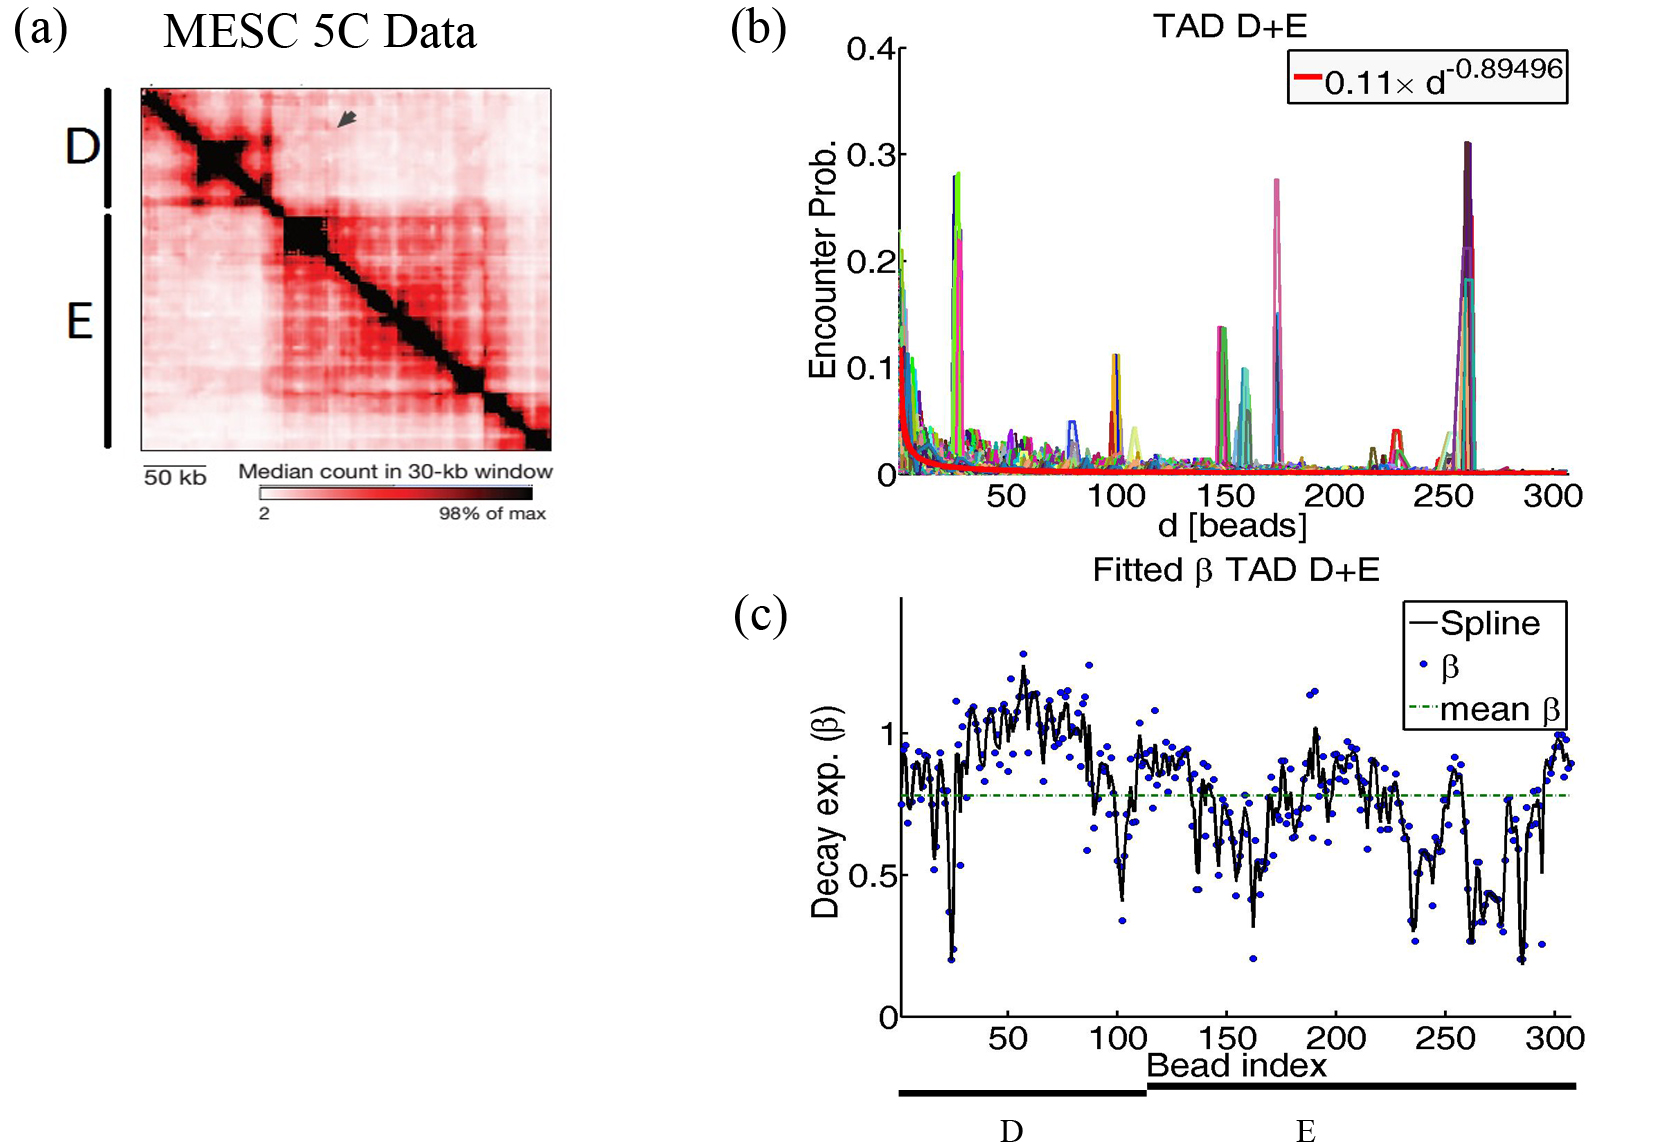
\includegraphics[scale=0.5]{Figure01_AnalysisOfTheExperimentalData}
\caption{\textbf{Analysis of the experimental data} (a) Average contact histogram of the 2 replicates of the 5C experiments in 2 discrete genomic regions of high self interactions termed TAD D and E (Nora et al \cite{Nora2012}) (b) The encounter probability graphs for each of the 307 beads show long range interactions between beads in TAD E and between TAD D and E, a fit of the form $\alpha d ^{-\beta}$ to the mean encounter of each distance (red curve), was found to have a decay exp. $\beta=0.729$, below the expected $\beta=1.5$ for a linear Rouse polymer, implying compact configuration of the polymer and looping (c) The calculated decay exp. value for each of the 307 beads (circles) was fitted with a smoothing spline (black curve) to show a fluctuating pattern around the mean ($\beta=0.729$, green dashed line) with sharp decrease in values for beads having long range interactions, e.g beads 25, 102, 165, 285.}
\label{figure_TADDAndENoraEtAl2012}
\end{figure}

\begin{figure}[H]
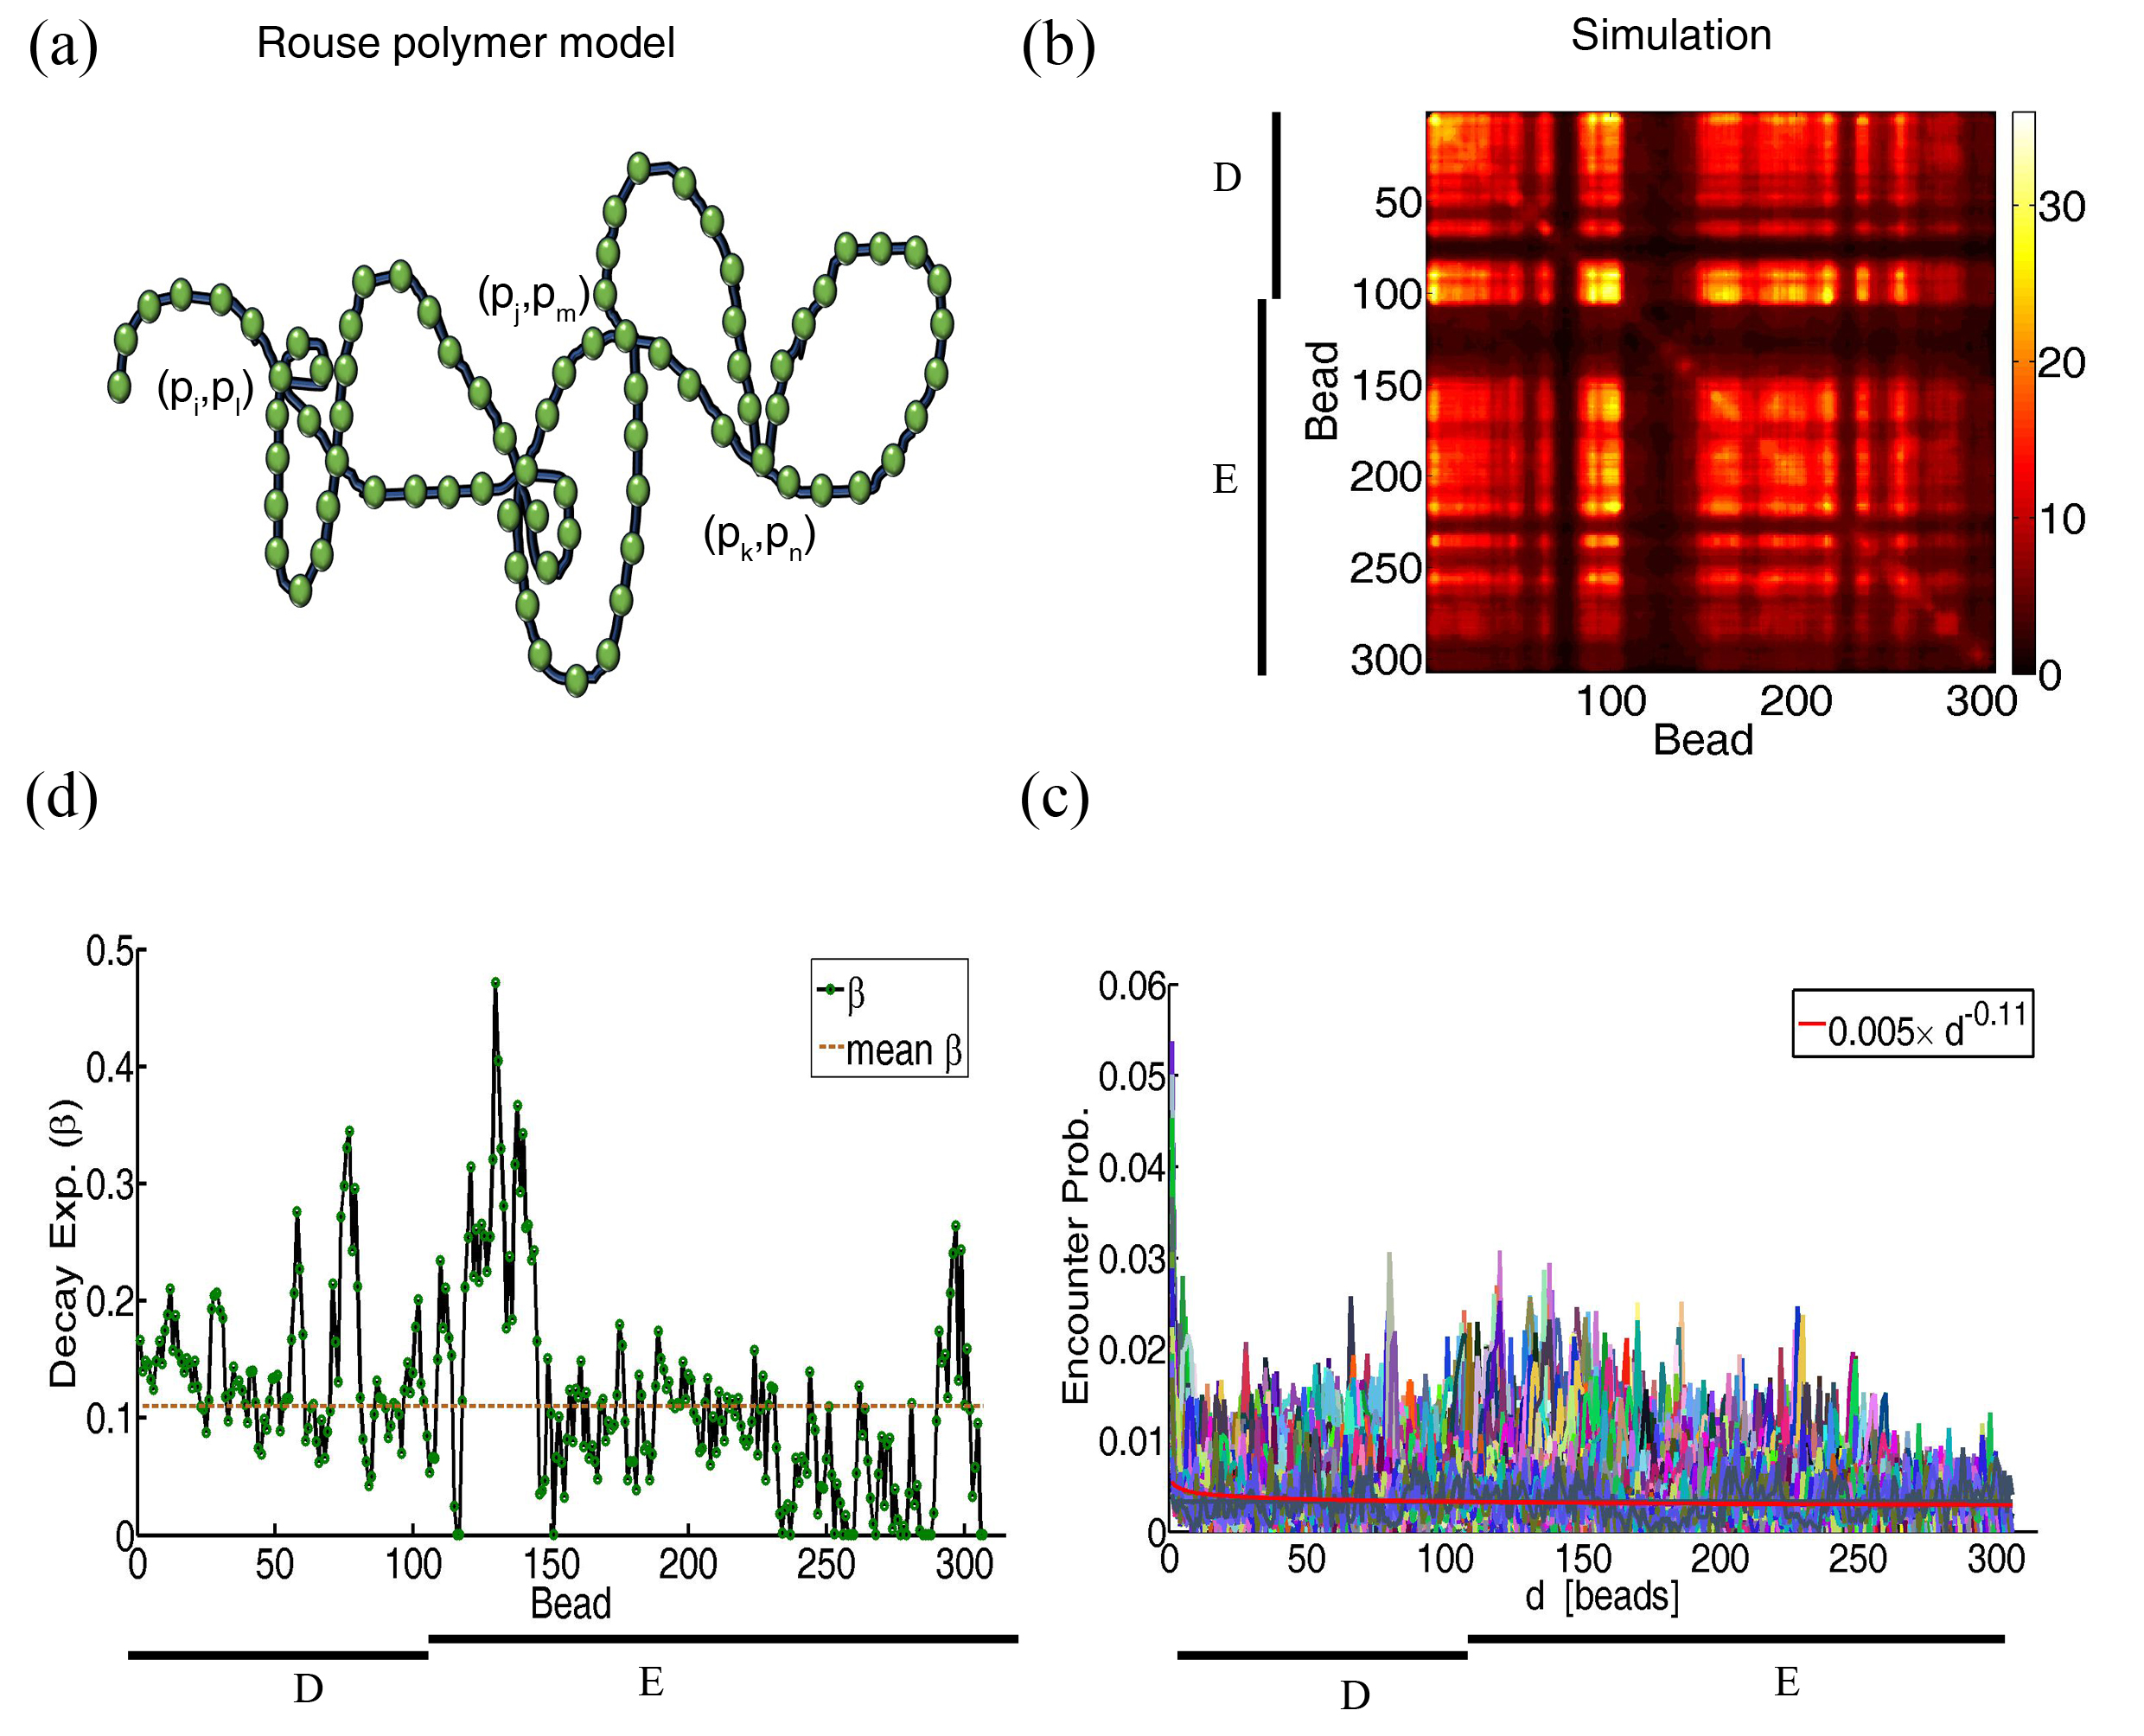
\includegraphics[scale=0.5]{Figure02_LoopsCorrespondingToPeaks307Beads}
\caption{\textbf{Simulation of a chain with connectors between beads corresponding to peaks of the encounter data}. (a) An illustration of a polymer connected between beads corresponding to peaks in the encounter data ($p_i,p_l), (p_j,p_m), (p_k,p_n)$ (b) The encounter histogram of the polymer with connectors does not show similarity to encounter histogram of the experimental data (Figure \ref{figure_TADDAndENoraEtAl2012}) (c) The encounter probabilities shows flat profile, indicating a compact polymer configuration. (d) the fitted decay exp. $\beta$ values for each one of the profiles in box (c) display low value corresponding to long range interaction of beads along the chain.)}
\label{figure_encounterProbabilityPeaksOfTheEncounterData}
\end{figure}

\begin{figure}[H]
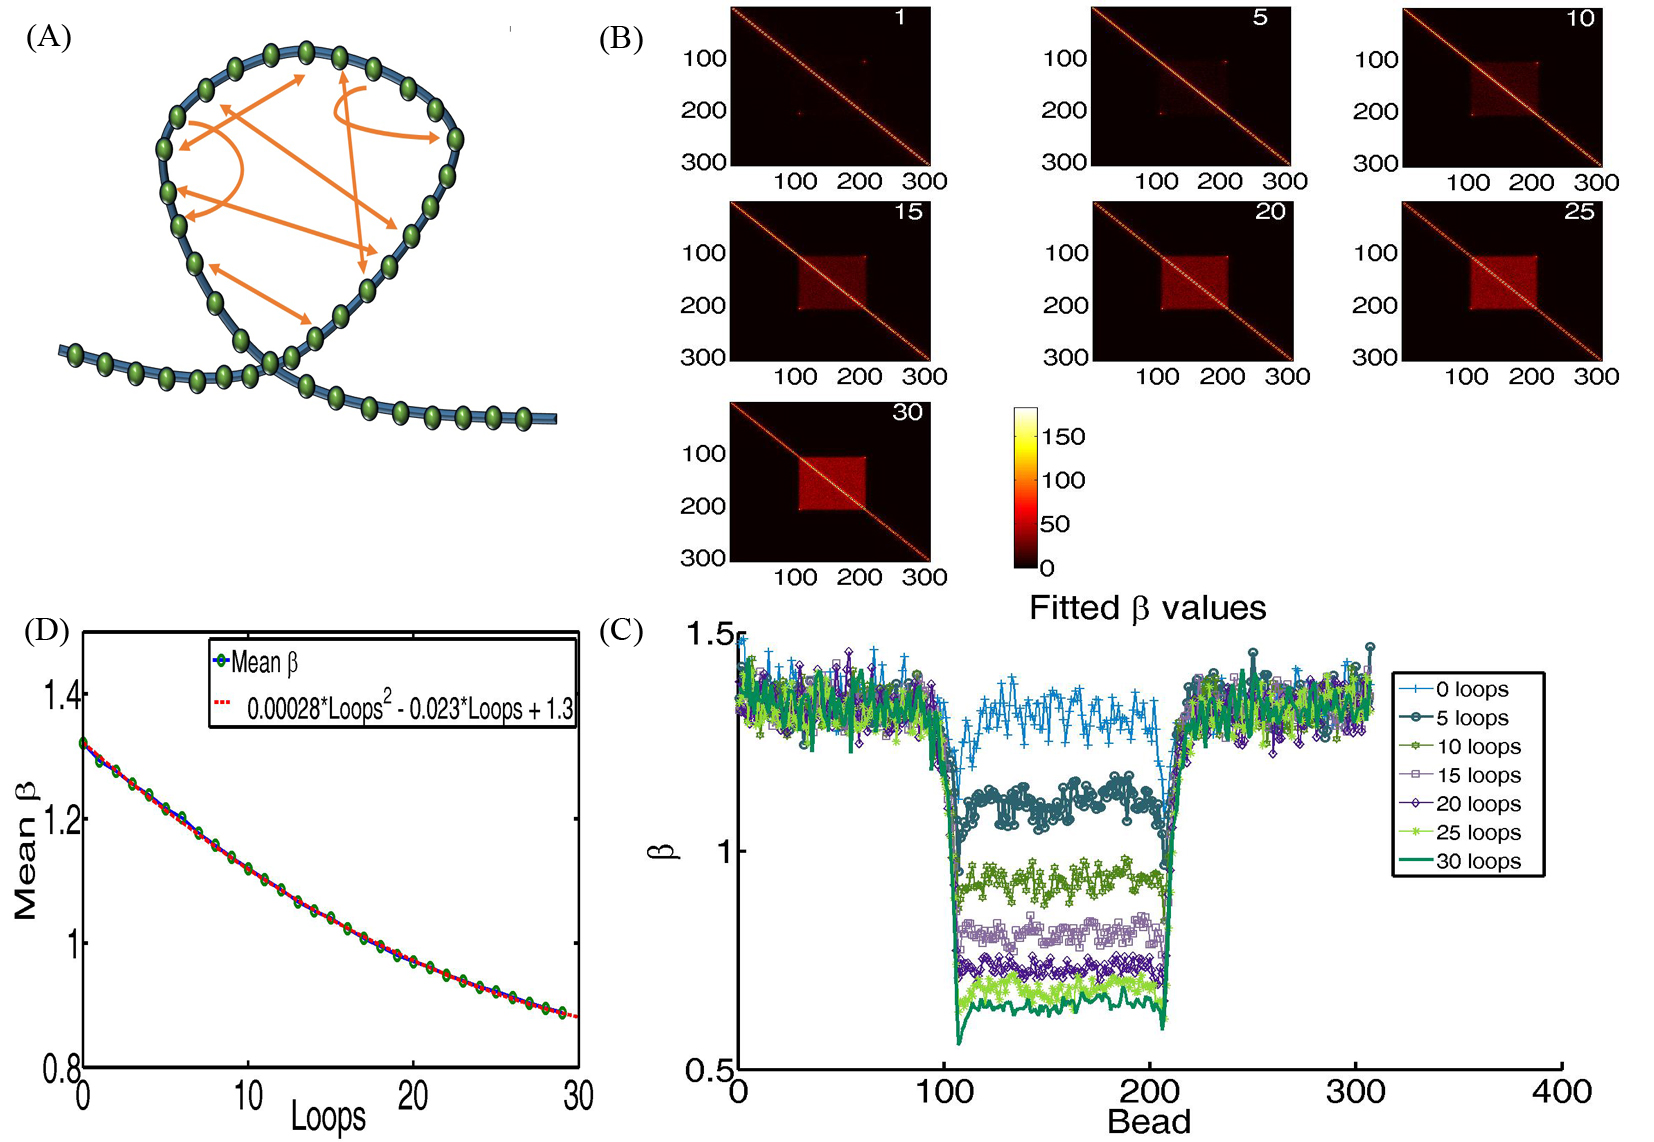
\includegraphics[scale=0.5]{Figure03_OneTADWithTails0To30RandomLoops}
\caption{\textbf{Encounter profile for a polymer model with one fixed loop and 1-30 random internal loops.} (a) A sketch of the polymer model used in simulation. Beads 107 and 207 were connected to form a 100 beads fixed loop, while 1 to 30 random internal loops were sequentially added. Each loop was formed by randomly picking a bead pair (orange arrow) in the range 108-206 (B) The encounter histograms for 7 cases (number of loops indicated in white) resembles a TAD region.(c) For each number of random internal loops, a model of the form $\alpha d^{-\beta}$ was fitted to the encounter probability of each bead, the resulting decay exp. $\beta$ values decreases sharply for beads in the loop range (107-207) with increased number of internal loops, whereas, beads outside the loop show similar behavior independent of the number of loops (D) The mean decay exp. $\beta$ values as a function of number of internal loops decreases quadratically and allows to infer from the measured mean encounter probability the number of loops in the polymer.}
\label{figure_encounterProfileOneTADWithTails}
\end{figure}

\begin{figure}[H]
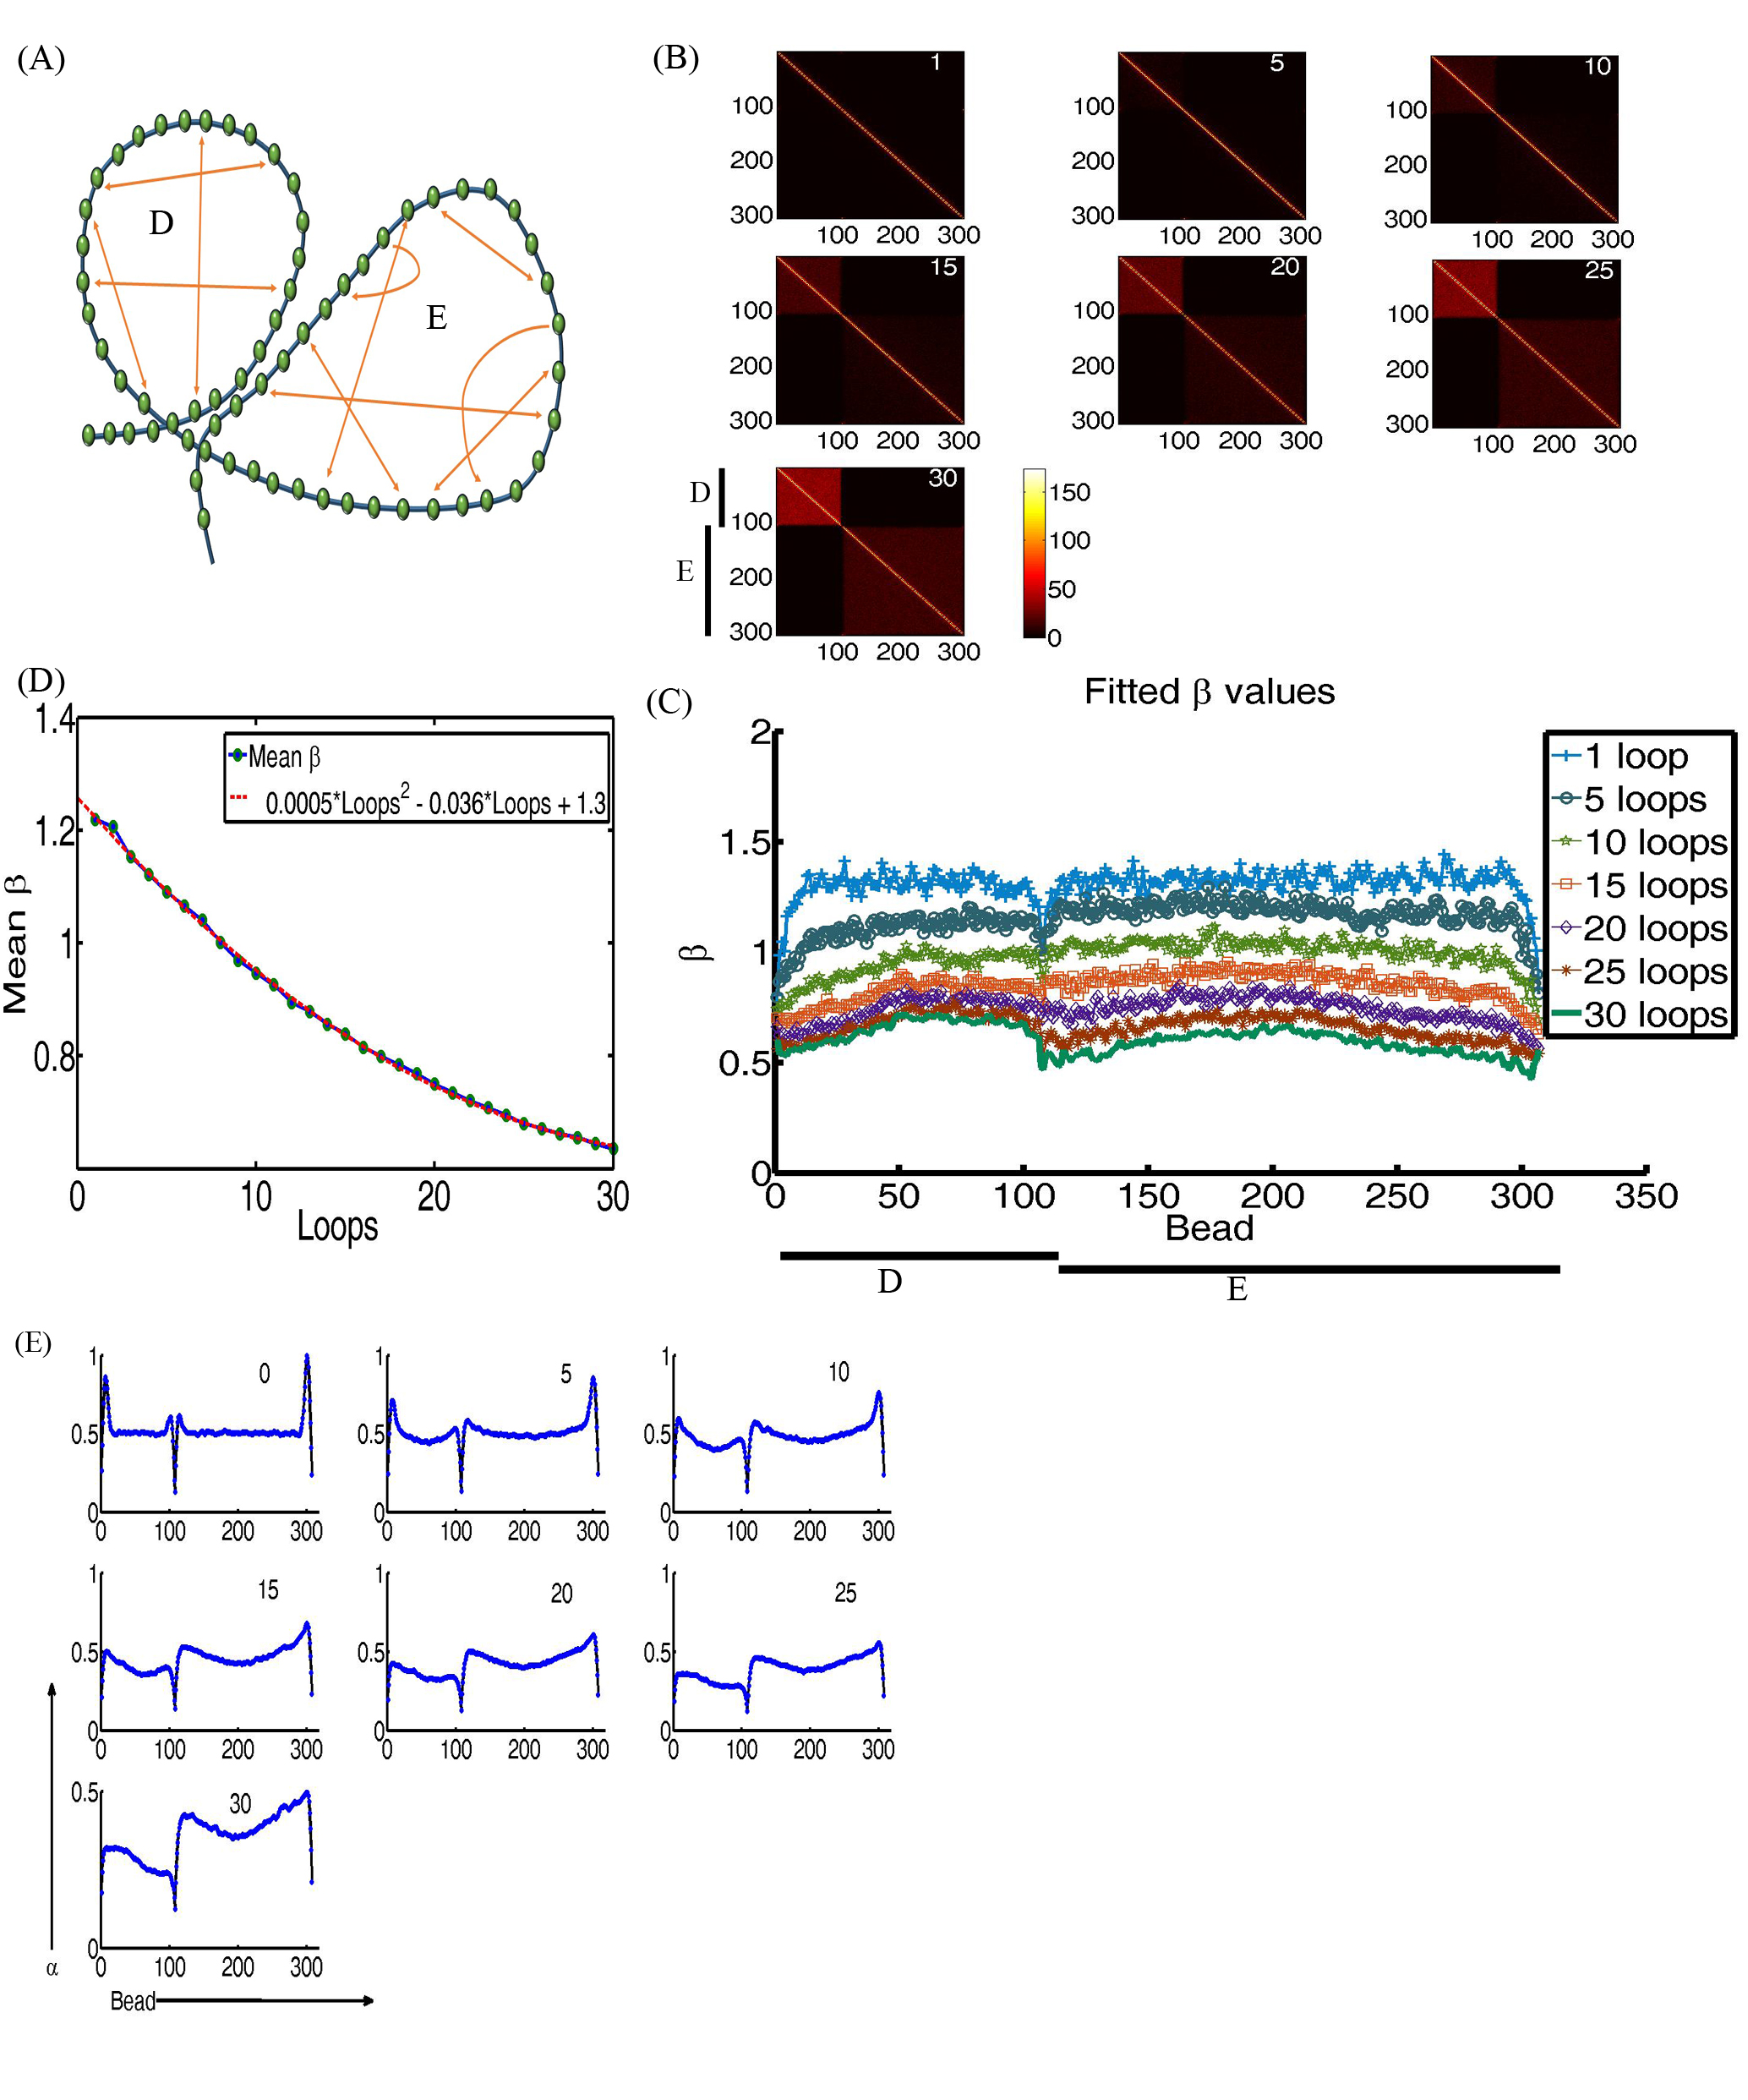
\includegraphics[scale=0.47]{Figure04_TwoTADs0To30RandomLoops307Beads}
\caption{\textbf{Encounter profile for a polymer model with two fixed loops and 1-30 random internal loops} (a) A sketch of the polymer model used in simulations. Beads 1,107 and beads 108,307 were connected to form two large loops corresponding to TAD D and E. One to 30 internal loops were sequentially added in each TAD (orange arrows) by randomly picking bead pairs in the range 2-106 and 108-306 (b) The encounter histograms for each number of loops (indicated in white in each box) resembles the TADs of the experimental data (Figure \ref{figure_TADDAndENoraEtAl2012}) as the number of loops increased. (c) For each number of internal loop, a model of the form $\alpha d^{-\beta}$ was fitted to the encounter probability of each bead. Beads on the edge between TADs (e.g beads 107, 108) show a decrease in the decay exponent due to frequent encounters with beads in both TADs. (d) A quadratic relationship was found empirically between the number of loops and the mean decay exp.(e) The anomalous exponent, $\alpha$, extracted from the fitted mean square displacement of each bead in the case of 0 to 30 random loops in each TAD.}
\label{figure_encounterProfileTwoTADs}
\end{figure}


\begin{figure}[H]
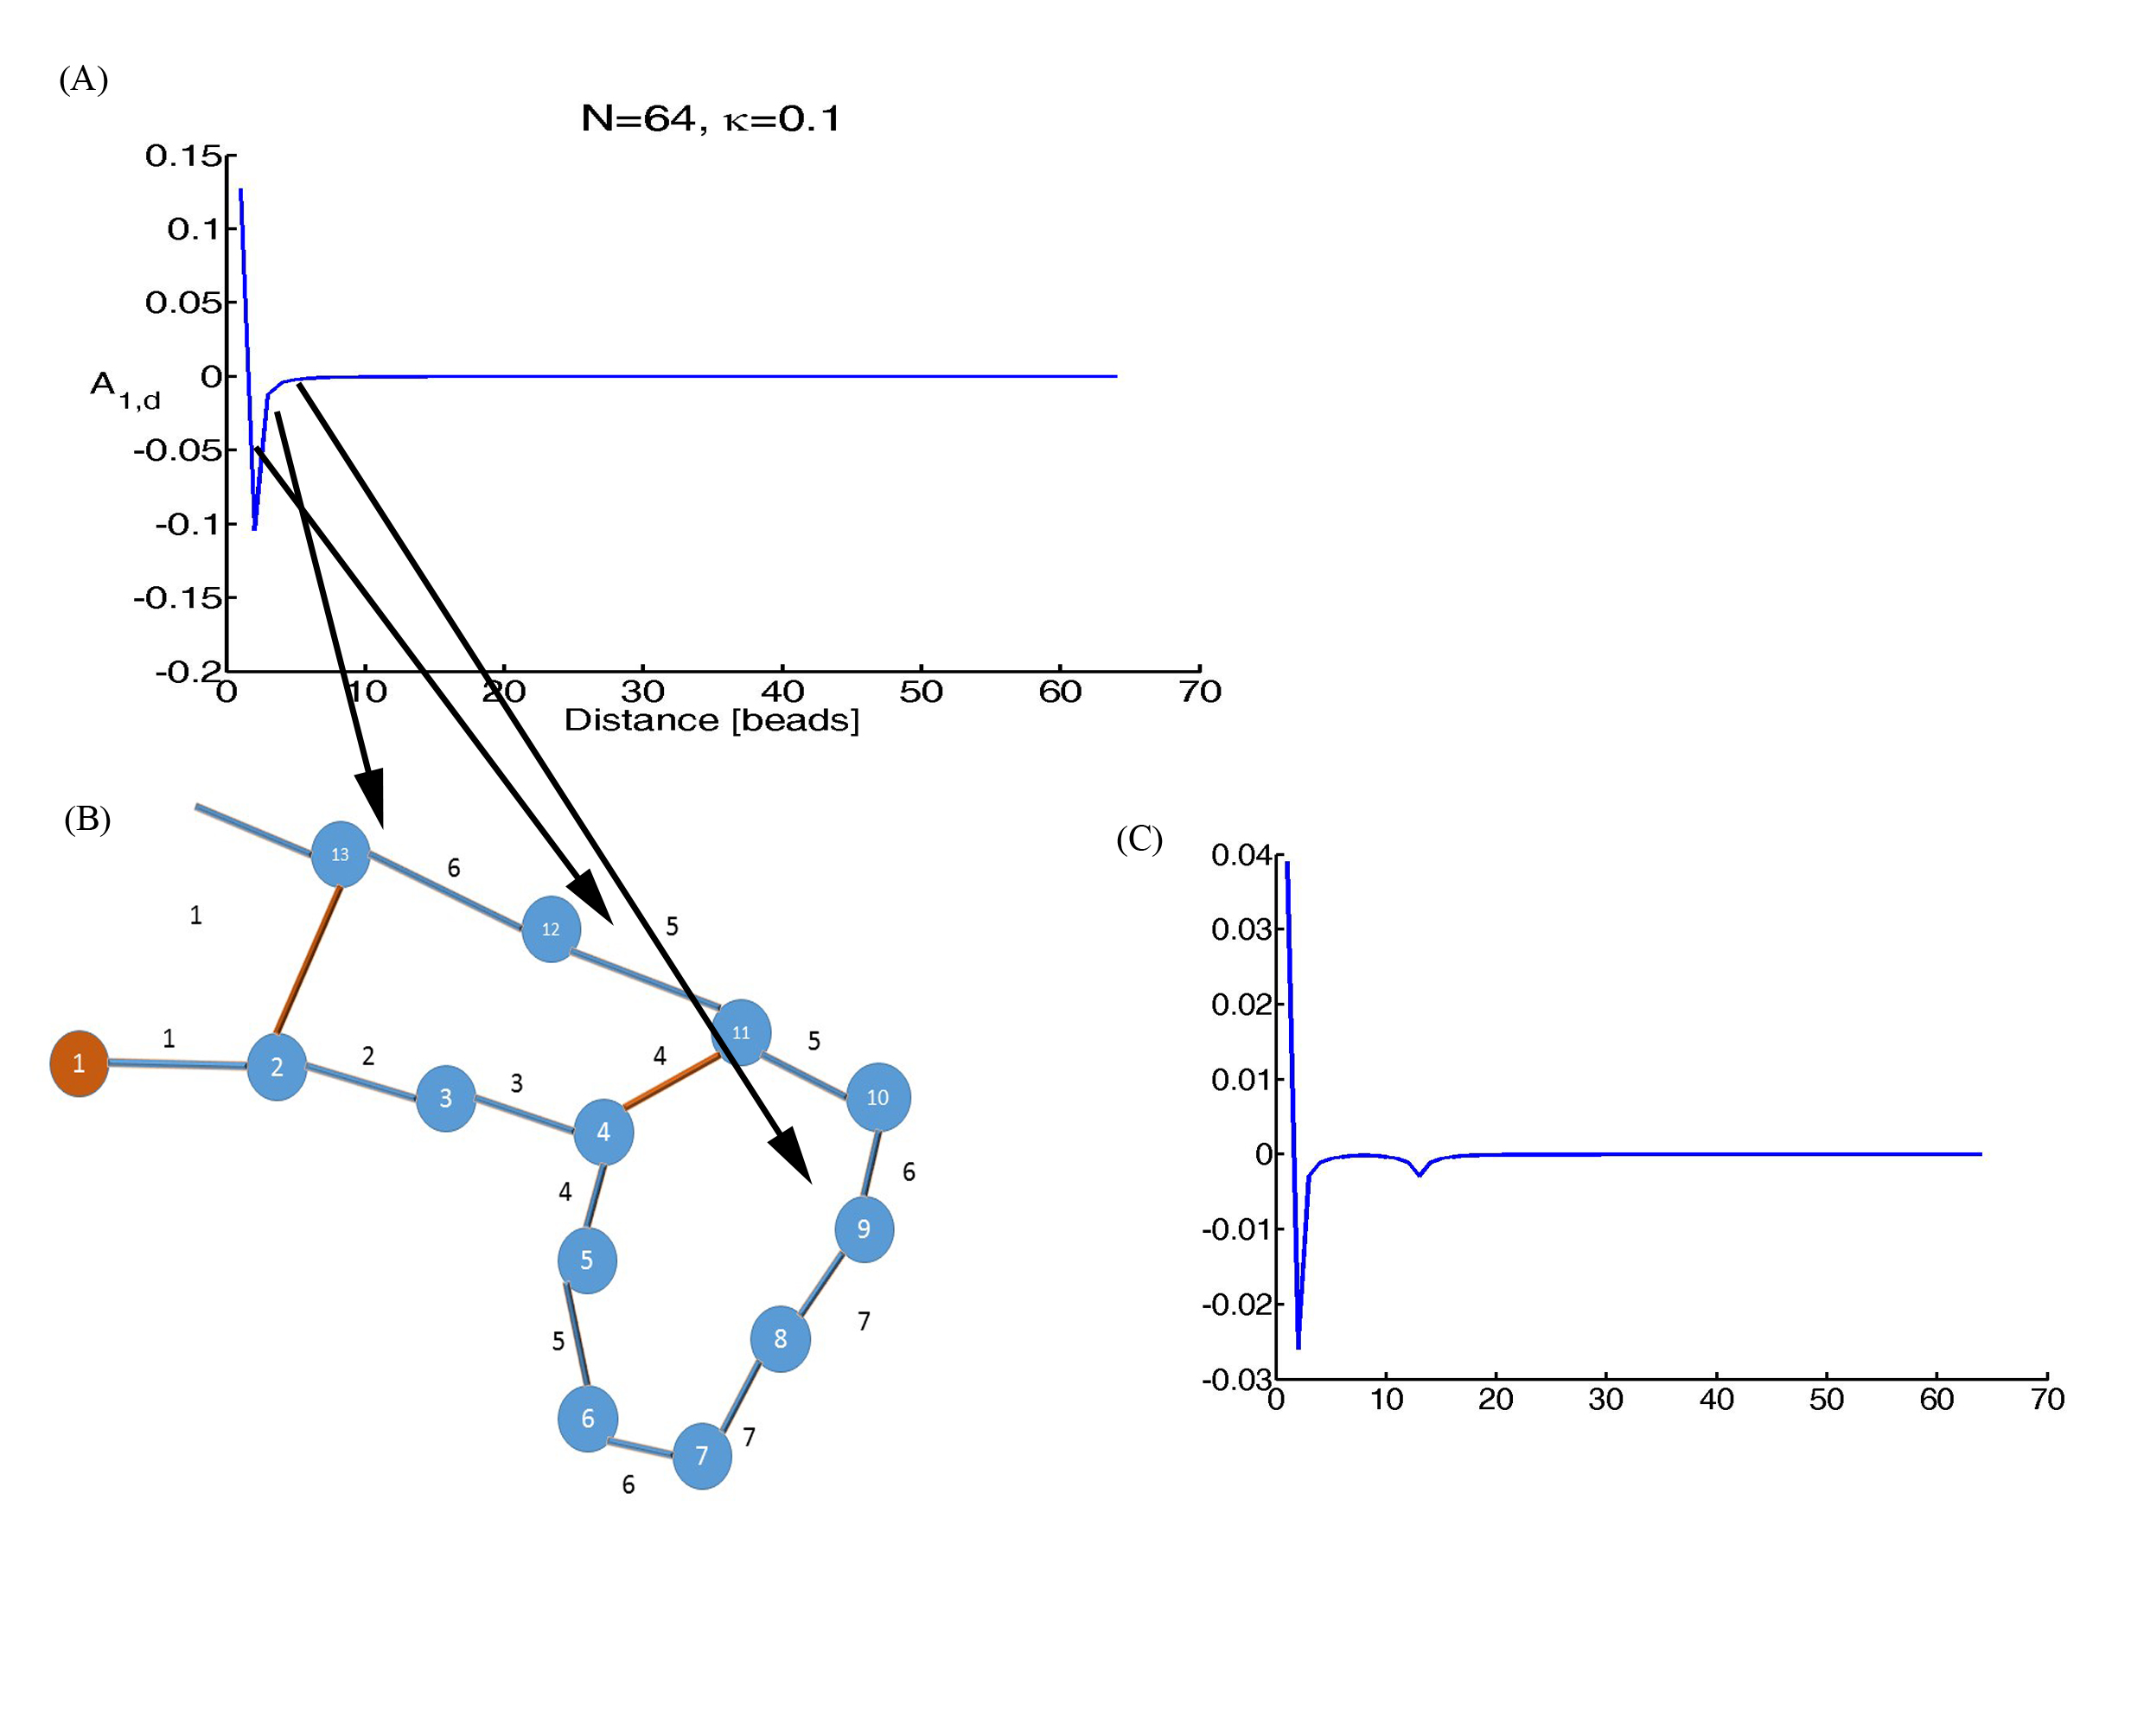
\includegraphics[scale=0.5]{Figure05_betaModelWeights}
\caption{\textbf{Setting the weights in the connectivity matrix of the $\beta$ polymer with loops}. (A) The weights in the matrix are determined by $A_{l,m}= 4\kappa \frac{2}{N}\sum_{p=1}^{N-1} sin^{\beta}(p\pi/(2N))cos((l-0.5)p\pi/N)\cos((m-0.5)p\pi/N)$, the curve is drawn for bead 1. (B) The polymer is treated as a graph with nodes representing beads (circles) and edges as springs (bars). An example of an architecture in which be beads 2 and 13 and 4 and 11 are connected (orange line). Arrows indicate that the new value for the weights for bead 1 in positions 13, 11, 9 are determined by the values of the original curve with no peaks at positions corresponding to the shortest distance on the graph between bead 1 to all others. (C) Connecting two beads in the polymer changes the weights  such that the new weights are assigned by the values of the $\beta$ polymer weights according to the closest distance between beads on the connected polymer graph.}
\label{settingBetsModelWeights}
\end{figure}

\begin{figure}[H]
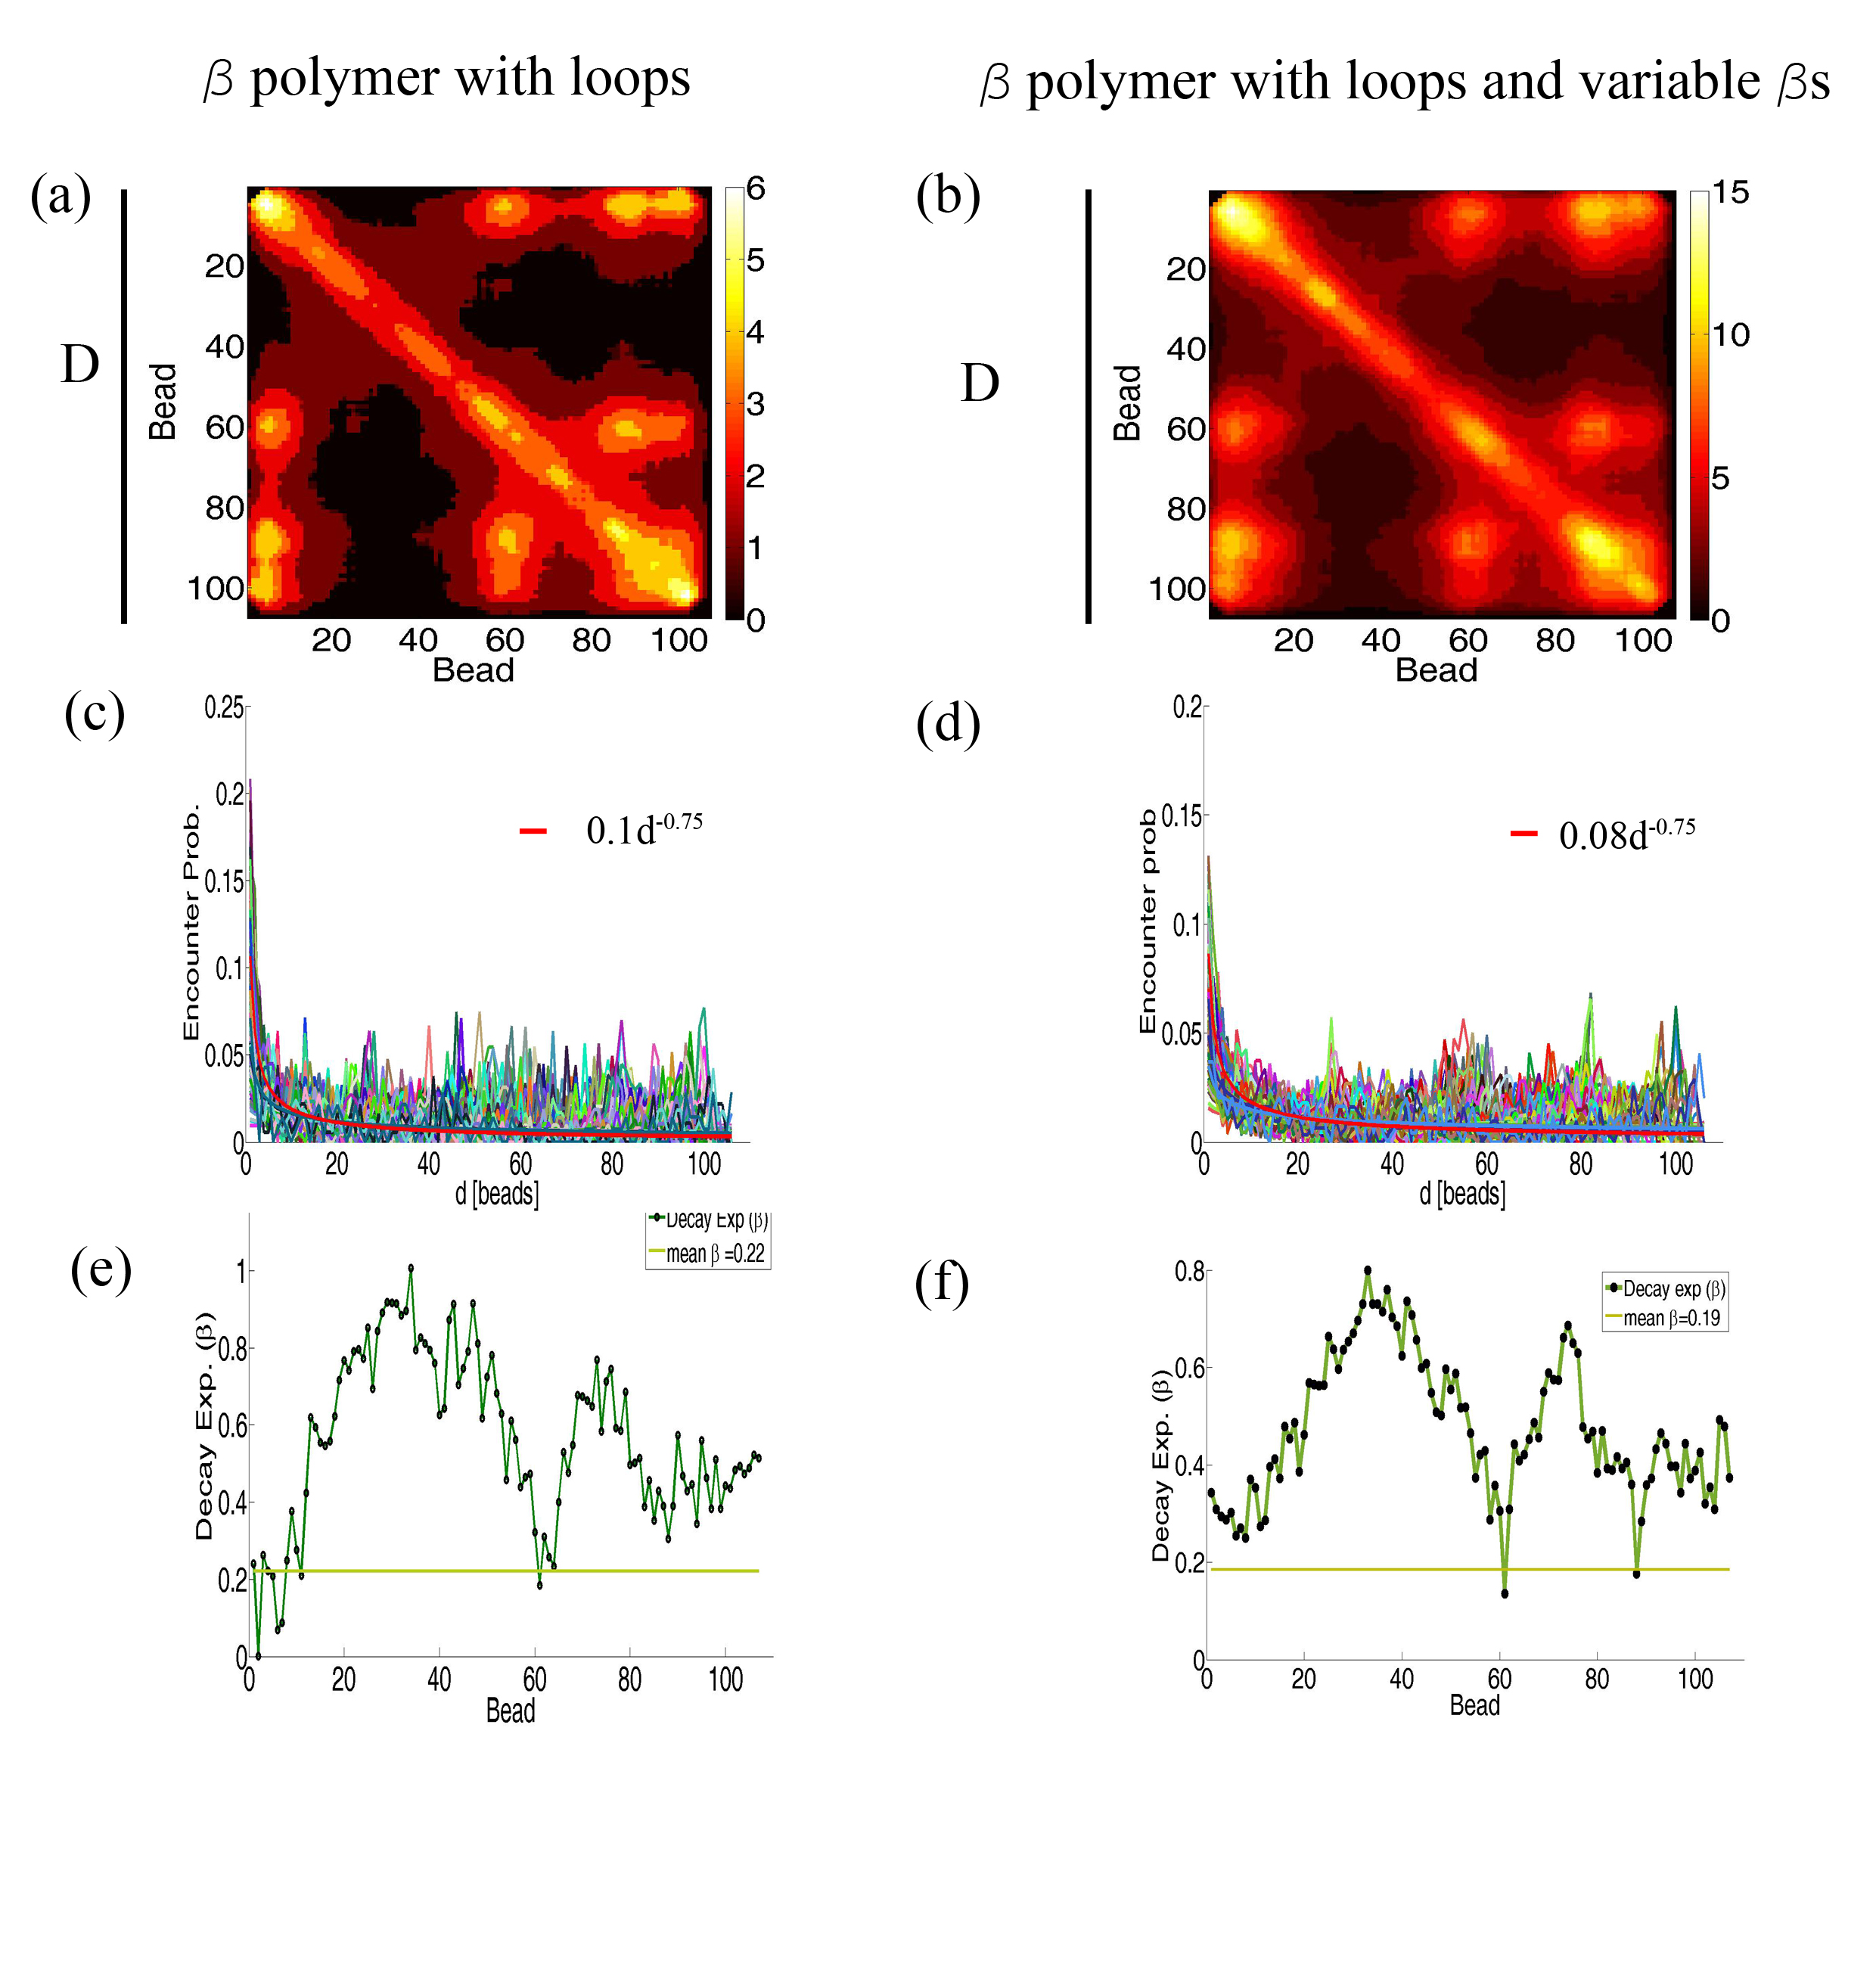
\includegraphics[scale=0.55]{Figure06_betaModelWithPeaks}
\caption{\textbf{A comparison between simulations of two $\beta$ models with loops corresponding to peaks of encounters in TAD D}. A uniform $\beta=1.5$ model (left column) was compared to a variable $\beta$ model (right column), with $\beta$ values extracted from the experimental data. Encounter histograms (a-b) showed similar qualitative behavior with slightly more contacts in the variable $\beta$ model, indicating a more compact configuration. This compaction was evident in the encounter probability signals (c-d) with a mean $\beta$ value (red curves) of 0.75 in the uniform vs. 0.67 is the variable model. A qualitatively similar behavior was noted in the fitted decay exponents values of each bead (e-f) and for the decay exponent of the average of the encounters (horizontal lines) of $0.22$ in the uniform vs $0.19$ of the variable $\beta$ model. Taken together, these observations suggest that a uniform $\beta$ value for all beads is enough to capture the complexity in the experimental data.}
\label{simulationWithBetaPolymerWithLoops}
\end{figure}

%> the bibliography section
\bibliographystyle{plain}
\bibliography{randomLoopsBibliography} % the bibliography.bib
\end{document}

